% NexPlay: documento final del Módulo V, Diplomado en Ciencia de Datos (FES Acatlán, UNAM).
% Se compila con LuaLaTeX y biber (ver .latexmkrc). Cada número del texto es una macro de
% tables/cifras.tex, que genera generar_figuras.py; ninguno se escribe a mano.
\documentclass[11pt]{article}

\usepackage[a4paper, margin=2.5cm]{geometry}
\usepackage{fontspec}
\setmainfont{Inter}
% Los nombres de código (endpoints, columnas, archivos) en monoespaciada, para distinguirlos del texto.
\setmonofont{DejaVu Sans Mono}[Scale=MatchLowercase]
% caption va antes de babel: sin él, babel en español y biblatex-apa chocan al cargar
% («Generic hooks cannot be added to '\@makecaption'»).
\usepackage{caption}
\usepackage[spanish, es-tabla]{babel}
\usepackage{csquotes}
\usepackage{xcolor}
\usepackage{graphicx}
\usepackage{booktabs}
\usepackage{tabularx}
\usepackage{float}
\usepackage{subcaption}
\usepackage{amsmath}
\usepackage{tikz}
\usetikzlibrary{arrows.meta, positioning}
\usepackage[style=apa, backend=biber]{biblatex}
\addbibresource{references.bib}
\usepackage[hidelinks]{hyperref}

\graphicspath{{figures/}}
\setlength{\parskip}{0.5em}
\setlength{\parindent}{0pt}
\linespread{1.1}
\captionsetup{font=small, labelfont=bf}
% Las tablas y figuras grandes se quedan arriba de una página con texto, en vez de dejar una
% página de flotantes con medio hueco; y TeX estira espacios antes de sacar una línea del margen.
\renewcommand{\topfraction}{0.9}
\renewcommand{\textfraction}{0.08}
\renewcommand{\floatpagefraction}{0.8}
\renewcommand{\arraystretch}{1.2}
\setlength{\emergencystretch}{2em}

% La paleta del frontend (tema claro, frontend/src/styles/tokens.css).
\definecolor{riesgobajo}{HTML}{047857}
\definecolor{riesgomedio}{HTML}{AA4F0A}
\definecolor{riesgoalto}{HTML}{BE123C}
\definecolor{acento}{HTML}{0E738F}
\definecolor{nia}{HTML}{6D28D9}
\definecolor{neutro}{HTML}{475585}

% Lo que todavía no tiene texto o evidencia se ve en el PDF, nunca se rellena.
\newcommand{\pendiente}[1]{\textcolor{riesgoalto}{\textbf{[PENDIENTE: #1]}}}
\newcommand{\pendienteEvidencia}{\textcolor{riesgoalto}{\textbf{[PENDIENTE DE EVIDENCIA]}}}
\newcommand{\pendienteColab}{\textcolor{riesgoalto}{\textbf{[PENDIENTE: corrida en Colab]}}}
% Las capturas se regeneran desde el tag de entrega; hasta entonces su pie lo dice.
\newcommand{\provisional}{\textit{Captura provisional: se regenera desde el tag de entrega.}}

% Generado por documento/generar_figuras.py. No se edita a mano.

\newcommand{\cifraJuegosEntrenamiento}{83}  % data-v1
\newcommand{\cifraResenasEntrenamiento}{123,972}  % data-v1
\newcommand{\cifraPositivosEntrenamiento}{2,714}  % data-v1: minutos < 120 y voto negativo
\newcommand{\cifraPrevalenciaEntrenamientoPorResena}{2.19\,\%}  % data-v1
\newcommand{\cifraJuegosCatalogo}{123}  % data-v3
\newcommand{\cifraResenasCatalogo}{184,367}  % data-v3
\newcommand{\cifraPositivosCatalogo}{4,126}  % data-v3: minutos < 120 y voto negativo
\newcommand{\cifraPrevalenciaCatalogoPorResena}{2.24\,\%}  % data-v3
\newcommand{\cifraJuegosExternos}{40}  % data-v3 sin los appids de data-v1
\newcommand{\cifraResenasExternos}{60,395}  % data-v3 sin los appids de data-v1
\newcommand{\cifraPositivosExternos}{1,412}  % data-v3 sin los appids de data-v1: minutos < 120 y voto negativo
\newcommand{\cifraPrevalenciaExternosPorResena}{2.34\,\%}  % data-v3 sin los appids de data-v1
\newcommand{\cifraPRAUCModelo}{0.0694}  % GroupKFold de 5 por appid sobre data-v1 (evaluar_gkf)
\newcommand{\cifraPRAUCModeloStd}{0.0415}  % GroupKFold de 5 por appid sobre data-v1 (evaluar_gkf)
\newcommand{\cifraPRAUCTrivial}{0.0219}  % GroupKFold de 5 por appid sobre data-v1 (evaluar_gkf); trivial = prevalencia de cada pliegue
\newcommand{\cifraPRAUCTrivialStd}{0.0037}  % GroupKFold de 5 por appid sobre data-v1 (evaluar_gkf)
\newcommand{\cifraPRAUCCociente}{3.17}  % GroupKFold de 5 por appid sobre data-v1 (evaluar_gkf)
\newcommand{\cifraPliegosGanados}{5}  % GroupKFold de 5 por appid sobre data-v1 (evaluar_gkf): pliegues donde el modelo supera al trivial
\newcommand{\cifraPliegues}{5}  % GroupKFold de 5 por appid sobre data-v1 (evaluar_gkf)
\newcommand{\cifraUmbralMedio}{0.2858}  % percentil 33.3 de los scores fuera de pliegue
\newcommand{\cifraUmbralAlto}{0.3916}  % percentil 66.7 de los scores fuera de pliegue
\newcommand{\cifraBajoEntrenamiento}{30}  % referencias/bandas_referencia.json
\newcommand{\cifraMedioEntrenamiento}{23}  % referencias/bandas_referencia.json
\newcommand{\cifraAltoEntrenamiento}{30}  % referencias/bandas_referencia.json
\newcommand{\cifraBajoCatalogo}{43}  % referencias/bandas_referencia.json
\newcommand{\cifraMedioCatalogo}{37}  % referencias/bandas_referencia.json
\newcommand{\cifraAltoCatalogo}{43}  % referencias/bandas_referencia.json
\newcommand{\cifraPRAUCExterno}{0.0356}  % docs/evidencia/prueba-externa.json
\newcommand{\cifraPRAUCExternoTrivial}{0.0234}  % docs/evidencia/prueba-externa.json
\newcommand{\cifraPRAUCExternoCociente}{1.52}  % docs/evidencia/prueba-externa.json
\newcommand{\cifraExternoICInf}{1.03}  % docs/evidencia/bootstrap-prueba-externa.json
\newcommand{\cifraExternoICSup}{2.33}  % docs/evidencia/bootstrap-prueba-externa.json
\newcommand{\cifraExternoReplicasSinVentaja}{27}  % réplicas del bootstrap con cociente ≤ 1
\newcommand{\cifraNovatosPorResena}{0.67\,\%}  % docs/evidencia/senal-por-biblioteca.json
\newcommand{\cifraNovatosPromJuegos}{0.97\,\%}  % docs/evidencia/senal-por-biblioteca.json
\newcommand{\cifraVeteranosPorResena}{2.89\,\%}  % docs/evidencia/senal-por-biblioteca.json
\newcommand{\cifraVeteranosPromJuegos}{2.72\,\%}  % docs/evidencia/senal-por-biblioteca.json
\newcommand{\cifraRazonMH}{2.62}  % docs/evidencia/senal-por-biblioteca-estratificada.json
\newcommand{\cifraRazonMHICInf}{1.84}  % docs/evidencia/senal-por-biblioteca-estratificada.json
\newcommand{\cifraRazonMHICSup}{4.12}  % docs/evidencia/senal-por-biblioteca-estratificada.json
\newcommand{\cifraDesdeJulioEntrenamientoPorResena}{96.1\,\%}  % data-v1: reseñas publicadas desde el 1 de julio de 2025 (UTC)
\newcommand{\cifraResenaMasAntiguaEntrenamiento}{8 de abril de 2023}  % data-v1: timestamp_created mínimo
\newcommand{\cifraResenaMasRecienteEntrenamiento}{14 de septiembre de 2026}  % data-v1: timestamp_created máximo
\newcommand{\cifraDescargaDesdeEntrenamiento}{14 de septiembre de 2026}  % data-v1: resenas.descargado_en mínimo
\newcommand{\cifraDescargaHastaEntrenamiento}{14 de septiembre de 2026}  % data-v1: resenas.descargado_en máximo
\newcommand{\cifraDesdeJulioCatalogoPorResena}{97.1\,\%}  % data-v3: reseñas publicadas desde el 1 de julio de 2025 (UTC)
\newcommand{\cifraResenaMasAntiguaCatalogo}{8 de abril de 2023}  % data-v3: timestamp_created mínimo
\newcommand{\cifraResenaMasRecienteCatalogo}{21 de septiembre de 2026}  % data-v3: timestamp_created máximo
\newcommand{\cifraDescargaDesdeCatalogo}{14 de septiembre de 2026}  % data-v3: resenas.descargado_en mínimo
\newcommand{\cifraDescargaHastaCatalogo}{21 de septiembre de 2026}  % data-v3: resenas.descargado_en máximo
\newcommand{\cifraTopeIngesta}{1,500}  % ingesta/ingesta_steam.py: MAX_RESENAS_POR_JUEGO
\newcommand{\cifraJuegosEnElTope}{81}  % data-v1: juegos con el tope de reseñas
\newcommand{\cifraDiasCubiertosMin}{4}  % data-v1: días entre la primera y la última reseña
\newcommand{\cifraDiasCubiertosMax}{1,252}  % data-v1: días entre la primera y la última reseña
\newcommand{\cifraDiasCubiertosMediana}{64}  % data-v1: mediana de días cubiertos
\newcommand{\cifraPrivadosEntrenamientoPorResena}{59.9\,\%}  % data-v1: num_games_owned = 0
\newcommand{\cifraSinNotaEntrenamiento}{23}  % data-v1: juegos sin nota de Metacritic
\newcommand{\cifraPagoSinPrecioEntrenamiento}{2}  % data-v1: juegos de pago sin precio
\newcommand{\cifraMetacriticVerificadoExternos}{40 de 40}  % docs/evidencia/verificacion-40-steam.csv


\begin{document}

\begin{titlepage}
    \begin{tikzpicture}[remember picture, overlay]
        \draw[line width=3pt, color=acento]
        ([shift={(1.2cm,-1.2cm)}]current page.north west)
        rectangle
        ([shift={(-1.2cm,1.2cm)}]current page.south east);
    \end{tikzpicture}

    \noindent
    \begin{minipage}{0.3\textwidth}
        \begin{flushleft}
            
\includegraphics[width=3.6cm]{escudos/logo_unam.png}
        \end{flushleft}
    \end{minipage}
    \hfill
    \begin{minipage}{0.3\textwidth}
        \begin{flushright}
            
\includegraphics[width=3.4cm]{escudos/logo_fes.png}
        \end{flushright}
    \end{minipage}

    \vspace*{2cm}

    \begin{center}
        {\LARGE Facultad de Estudios Superiores Acatlán} \\[0.8cm]
        {\LARGE Diplomado en Ciencia de Datos} \\[0.8cm]
        {\LARGE Módulo V} \\[2cm]
        {\Huge \textbf{Proyecto final}} \\[1cm]
        {\Large NexPlay: señal de arrepentimiento temprano} \\[0.3cm]
        {\Large antes de comprar un videojuego} \\[2.5cm]
        {\LARGE \textbf{Fernando Axel Ramírez Gómez}} \\[0.8cm]
        {\Large \today}
    \end{center}
\end{titlepage}

% Rúbrica: Introducción (abstract claro y conciso, en lenguaje accesible para un público general).
\section*{Resumen}
\addcontentsline{toc}{section}{Resumen}

\preguntaguia{} Esa es la pregunta que NexPlay ayuda a contestar. Steam deja devolver un videojuego
si se ha jugado menos de dos horas, y NexPlay usa ese límite: cuenta, en cada juego, las reseñas
negativas escritas antes de las dos horas, una señal de que el juego decepcionó pronto. Con \cifraResenasEntrenamiento{} reseñas de
\cifraJuegosEntrenamiento{} juegos se entrenó un modelo sencillo que estima qué juegos dejan más
de esa señal usando solo lo que cualquiera ve en la tienda antes de pagar: si el juego es gratis,
su precio, su descuento y la nota de la crítica. El modelo distingue a esos juegos mejor que un
clasificador que no sabe nada, también en \cifraJuegosExternos{} juegos que no vio, aunque la
ventaja es modesta. El sitio no da probabilidades ni dice qué comprar: da un riesgo de
arrepentimiento bajo, medio o alto; explica qué lo mueve y de qué se quejan las reseñas; deja
comparar juegos y preguntarle a un asistente, y recuerda la ventana de reembolso. Es una segunda
opinión antes de pagar. Un análisis aparte, con modelos que leen las reseñas, mostró que esas quejas tempranas
tienen un lenguaje propio: hablan de entrar al juego, del rendimiento y del reembolso. El riesgo,
sin embargo, sale solo de datos del juego y es el mismo para cualquier persona.


\tableofcontents
\newpage

% Rúbrica: Introducción. Fuentes y figuras: ver el plan del documento.
\section{Introducción}\label{sec:introduccion}

\subsection{Contexto}
\pendiente{redacción}

\subsection{Preguntas del proyecto}
\pendiente{redacción}

\subsection{Qué entrega el proyecto}
\pendiente{redacción}

\subsection{Mapa del documento contra la rúbrica}
\pendiente{redacción}

% Rúbrica: Planteamiento del problema. Fuentes y figuras: ver el plan del documento.
\section{Planteamiento del problema}\label{sec:planteamiento}

\subsection{La decisión antes de pagar}
\pendiente{redacción}

\subsection{Por qué el promedio de reseñas no basta}
\pendiente{redacción}

\subsection{Qué se puede observar y qué no}
\pendiente{redacción}

% Rúbrica: Estrategia (usuarios). Fuentes y figuras: ver el plan del documento.
\section{Nicho de negocio y usuario final}\label{sec:nicho}

\subsection{Una capa previa a la compra}
\pendiente{redacción}

\subsection{El usuario, por comportamiento}
\pendiente{redacción}

\subsection{Veteranos y novatos}
\pendiente{redacción}

% Rúbrica: Estrategia (15 puntos). Fuentes y figuras: ver el plan del documento.
\section{Estrategia: accionables, usuarios y usabilidad}\label{sec:estrategia}

\subsection{Accionables}
\pendiente{redacción}

\subsection{Usuarios y necesidades}
\pendiente{redacción}

\subsection{Recorrido: PAYDAY 3 contra Dead Space}
\pendiente{redacción}

\subsection{Usabilidad}
\pendiente{redacción}

% Rúbrica: Descripción de los datos. Fuentes y figuras: ver el plan del documento.
\section{Descripción de los datos}\label{sec:datos}

\subsection{La API de Steam}
\pendiente{redacción}

\subsection{Releases y su verificación}
\pendiente{redacción}

\subsection{Periodo que cubren}
\pendiente{redacción}

\subsection{Calidad}
\pendiente{redacción}

% Rúbrica: Análisis exploratorio y modelación (la variable objetivo y su métrica).
\section{Definición del objetivo}\label{sec:objetivo}

El modelo aprende a ordenar juegos según una señal que sale de sus reseñas: un voto negativo
escrito antes de las dos horas de juego. Esa señal no es el arrepentimiento mismo, el corte de
120 minutos viene de una regla de Steam y la métrica tiene que funcionar con una clase muy rara.

\subsection{La fórmula}\label{sec:objetivo-formula}

Para cada reseña $i$,
\[
  Y_i =
  \begin{cases}
    1 & \text{si } \texttt{playtime\_at\_review}_i < 120 \text{ y } \texttt{voted\_up}_i = 0,\\
    0 & \text{en otro caso,}
  \end{cases}
\]
donde \texttt{playtime\_at\_review} son los minutos que llevaba jugados quien escribió la reseña
cuando la publicó y \texttt{voted\_up} es el pulgar: 1 arriba, 0 abajo. En data-v1 hay
\cifraPositivosEntrenamiento{} reseñas con $Y = 1$ de \cifraResenasEntrenamiento{}, una
prevalencia de \cifraPrevalenciaEntrenamientoPorResena{} por reseña. A esa etiqueta se le llama
\emph{señal de arrepentimiento temprano}.

\subsection{Por qué es una señal proxy}\label{sec:objetivo-proxy}

Steam no registra arrepentimiento. Registra que alguien votó en contra y cuánto había jugado al
escribir. Los 120 minutos vienen de la política de reembolsos de la tienda: se puede pedir el
reembolso dentro de las dos semanas posteriores a la compra y con menos de dos horas de juego
\parencite{steam_reembolsos}. Una reseña negativa escrita dentro de esa ventana es lo más cercano
que dejan los datos a «esto no era para mí, y me di cuenta pronto».

Por eso el sitio y este documento la llaman señal de arrepentimiento temprano y nunca dicen que
alguien se arrepintió. La señal deja fuera a quien se arrepiente y no escribe, a quien pide el
reembolso sin reseñar y a quien reseña después de las dos horas. Tampoco mide abandono ni
reembolsos: de ninguno de los dos hay dato.

Lo que sí muestran los datos es que las negativas llegan antes. El
\cifraNegativasAntesDelUmbralPorResena{} de las reseñas negativas se escribe antes de los 120
minutos, contra el \cifraPositivasAntesDelUmbralPorResena{} de las positivas. La señal se queda con
ese tramo temprano de las negativas.

\subsection{Robustez del umbral de 120 minutos}\label{sec:objetivo-umbral}

El umbral no se eligió con los datos, sale de la regla de Steam. Lo que sí se revisó es si
moverlo cambia qué juegos tienen más señal. Con 60, 90 o 180 minutos cambia cuántas reseñas
cuentan, pero el orden de los juegos casi no se mueve: su correlación de Spearman con el orden de
120 va de \cifraSpearmanUmbralMin{} a \cifraSpearmanUmbralMax{} (tabla~\ref{tab:umbral}).

\begin{table}[htbp]
  \centering\small
  % Generado por documento/generar_figuras.py. No se edita a mano.
\begin{tabular}{rrrr}
\toprule
Umbral (min) & Reseñas con señal & Prevalencia por reseña & Spearman con 120 (por juego) \\
\midrule
60 & 1,649 & 1.33\,\% & 0.964 \\
90 & 2,250 & 1.81\,\% & 0.989 \\
120 & 2,714 & 2.19\,\% & 1.000 \\
180 & 3,349 & 2.70\,\% & 0.993 \\
\bottomrule
\end{tabular}

  \caption{La señal con otros umbrales. La prevalencia es por reseña; el Spearman compara las
  tasas por juego de los \cifraJuegosEntrenamiento{} juegos contra las de 120 minutos. Fuente:
  data-v1, con \texttt{sensibilidad\_umbral} de \texttt{analisis/exploracion.py}.}
  \label{tab:umbral}
\end{table}

La figura~\ref{fig:minutos} muestra en qué minuto se escribe cada reseña. En 120 no hay escalón:
por minuto, las negativas pasan de \cifraNegativasPorMinutoAntesDelUmbral{} a
\cifraNegativasPorMinutoDespuesDelUmbral{} al cruzarlo, y las positivas de
\cifraPositivasPorMinutoAntesDelUmbral{} a \cifraPositivasPorMinutoDespuesDelUmbral{}. El salto
que se ve está en los 180 minutos y solo en las positivas, que pasan de
\cifraPositivasPorMinutoAntesDeTresHoras{} a \cifraPositivasPorMinutoDesdeTresHoras{} reseñas por
minuto en \cifraJuegosSaltoTresHoras{} juegos. Las negativas apenas cambian (de
\cifraNegativasPorMinutoAntesDeTresHoras{} a \cifraNegativasPorMinutoDesdeTresHoras{}). La causa de
ese salto no está en estos datos, y no toca la señal, que se define en 120 minutos y con reseñas
negativas.

\begin{figure}[htbp]
  \centering
  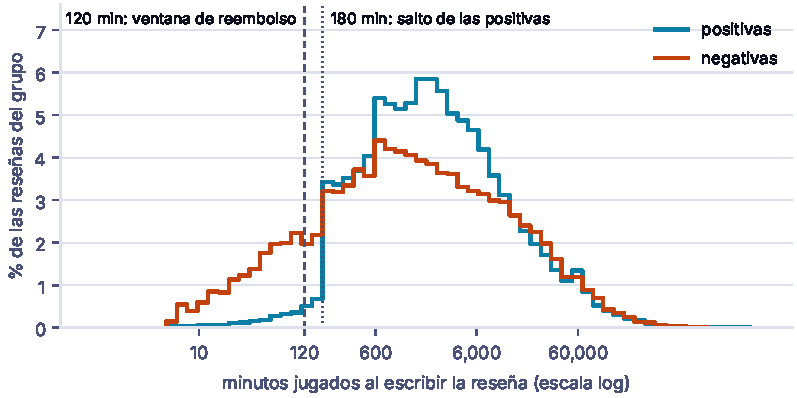
\includegraphics[width=\textwidth]{minutos-al-resenar.pdf}
  \caption{Minutos jugados al escribir la reseña, por pulgar, en escala logarítmica. Cada curva
  se normaliza sobre su propio grupo. Los intervalos tienen el mismo ancho en escala log, con un borde en 180
  y ninguno en 120. Fuente: data-v1.}
  \label{fig:minutos}
\end{figure}

\subsection{Por qué PR-AUC}\label{sec:objetivo-metrica}

Con una prevalencia de \cifraPrevalenciaEntrenamientoPorResena{}, un modelo que siempre dice «no»
acierta el \cifraExactitudTrivialPorResena{} de las veces y no encuentra un solo caso. La
exactitud premia justo eso, así que aquí no sirve. El proyecto usa el área bajo la curva de
precisión y exhaustividad (PR-AUC, con \texttt{average\_precision\_score} de scikit-learn). Mide
qué proporción de lo que el modelo pone arriba es de verdad señal, y con clases desbalanceadas informa
más que la curva ROC \parencite{saito2015,davis2006}.

El PR-AUC de un clasificador que no sabe nada es la prevalencia, \cifraPRAUCTrivial{}. Ese es el
piso, y por eso en este documento el PR-AUC del modelo siempre va junto al del trivial. En la
validación agrupada por juego el modelo llega a \cifraPRAUCModelo{}, \cifraPRAUCCociente{} veces
ese piso (sección~\ref{sec:evaluacion}).

% Rúbrica: Análisis exploratorio de datos. Fuentes y figuras: ver el plan del documento.
\section{Análisis exploratorio}\label{sec:exploracion}

\subsection{La tasa varía por juego}
\pendiente{redacción}

\subsection{La crítica acompaña a la señal}
\pendiente{redacción}

\subsection{El texto de las negativas tempranas}
\pendiente{redacción}

\subsection{Los 83 contra los 40}
\pendiente{redacción}

% Rúbrica: Procesamiento de datos. Fuente: notebooks/00_exploracion.ipynb, bloques 1 y 2, §3.5, y
% backend/analisis/limpieza.py.
\section{Procesamiento de datos}\label{sec:procesamiento}

El procesamiento tiene dos destinos. El modelo de riesgo se entrena con data-v1 tal como se
publicó, porque solo usa variables del juego y no lee texto. La limpieza produce otro conjunto,
el limpio, que usan el análisis de texto (sección~\ref{sec:exploracion-texto}) y la medición de
los motivos (sección~\ref{sec:interpretabilidad-motivos}).

\subsection{Validación}\label{sec:procesamiento-validacion}

Antes de todo, el notebook 00 corre los chequeos de la tabla~\ref{tab:calidad}
(sección~\ref{sec:datos-calidad}). Los de rango que nunca deben fallar, como un minuto negativo
o un voto distinto de 0 y 1, son aserciones\footnote{Una aserción es una comprobación dentro del
código: si no se cumple, la ejecución se detiene con un error.}, así que el notebook no sigue si
uno falla. También se revisan las copias que cruzan la partición: \cifraTextosEntreJuegos{}
textos idénticos, de \cifraPalabrasDeUnaCopia{} palabras o más, aparecen en más de un juego, y
\cifraCopiasEnFoldsDistintos{} de ellos quedan en folds distintos. Un modelo de texto podría
verlos en entrenamiento y en prueba, y por eso la limpieza quita los duplicados. La partición
misma está congelada en un archivo (sección~\ref{sec:modelacion-validacion}).

\subsection{Limpieza: marcar, no borrar}\label{sec:procesamiento-limpieza}

Cada regla es una función de \texttt{backend/analisis/limpieza.py}, y se aplican en el orden de
la tabla~\ref{tab:limpieza}. Solo dos quitan filas: los textos idénticos, de los que se queda la
reseña más antigua, y las reseñas vacías. Los duplicados quitan \cifraDuplicadosQuitados{}
filas y las vacías \cifraVaciasQuitadas{}, y quedan \cifraResenasLimpias{} reseñas. Las demás reglas agregan
una columna que marca la reseña y la dejan en su lugar. Las cortas, por ejemplo, son el
\cifraCortasPorResena{} de las reseñas, y quitarlas cambiaría qué reseñas se estudian, no solo
cuánto ruido hay. La normalización pasa el texto a minúsculas, quita el BBCode\footnote{El
formato que Steam permite en las reseñas, con etiquetas como \texttt{[h1]} o
\texttt{[spoiler]}.} y las direcciones web, y abre las contracciones: «don't» queda como «do
not», y la negación, como palabra suelta.

\begin{table}[htbp]
  \centering\small
  % Generado por documento/generar_figuras.py. No se edita a mano.
\begin{tabularx}{\textwidth}{>{\raggedright\arraybackslash}X >{\raggedright\arraybackslash}p{4.4cm} rr}
\toprule
Regla, en orden & Qué se hace & Afectadas & Quedan \\
\midrule
Texto idéntico de 8 palabras o más & se quitan; queda la más antigua & 483 (0.4\,\%) & 123,489 \\
Reseña vacía & se quitan & 545 (0.4\,\%) & 122,944 \\
Menos de 3 palabras & se marcan & 27,944 (22.7\,\%) & 122,944 \\
Otro idioma, según lingua & se marcan & 1,637 (1.3\,\%) & 122,944 \\
Plantilla de casillas & se marcan & 191 (0.2\,\%) & 122,944 \\
Normalización del texto & se agrega \texttt{texto\_norm} & 94,303 (76.7\,\%) & 122,944 \\
\bottomrule
\end{tabularx}

  \caption{Bitácora de la limpieza sobre data-v1. El porcentaje es sobre las reseñas que llegan a
  cada regla; en la normalización, las afectadas son las que cambian de texto. Fuente:
  \texttt{limpiar} de \texttt{backend/analisis/limpieza.py}.}
  \label{tab:limpieza}
\end{table}

La limpieza no se aplica al modelo de riesgo. Se midió qué le pasaría con la misma partición
congelada, para que la diferencia saliera de las filas y no del reparto de los juegos. Sin los
duplicados, su PR-AUC pasa de \cifraPRAUCModelo{} a \cifraPRAUCSinDuplicados{}, y sin las
vacías, a \cifraPRAUCSinVacias{}. Sin las cortas subiría a \cifraPRAUCSinCortas{}, pero sobre
otra población y con más prevalencia, así que los dos números no se comparan. El modelo se queda
con data-v1 tal cual. El conjunto limpio se guarda con un sha256 de su contenido, y quien lo
rehaga puede comprobar que obtuvo el mismo.

\subsection{Idioma}\label{sec:procesamiento-idioma}

La ingesta pidió reseñas en inglés (\texttt{language=english}), y Steam entrega las que llevan
esa etiqueta. Para revisarla se usó lingua\footnote{Una biblioteca de detección de idioma. Solo
decide cuando tiene confianza; los textos muy cortos o sin sentido quedan como
indeterminados.}: el \cifraIdiomaInglesPorResena{} de las reseñas limpias está en inglés o no se
pudo determinar, y \cifraOtroIdioma{} están escritas en otro idioma, sobre todo ruso, español y
portugués. Como el filtro lo aplicó Steam, esa cifra mide qué tan bien etiquetaron sus reseñas
los autores, no qué idiomas se usan en la tienda. Las reseñas en otro idioma se marcan y se
quedan. Al modelo de riesgo no le afectan, porque no lee texto, pero a los motivos sí, porque sus
palabras clave están en inglés (sección~\ref{sec:interpretabilidad-motivos}).

\subsection{Precio imputado}\label{sec:procesamiento-precio}

Los \cifraPagoSinPrecioEntrenamiento{} juegos de pago que llegaron sin precio
(tabla~\ref{tab:calidad}) entran al modelo con precio 0: la variable es el logaritmo de uno más
el precio, y los faltantes se llenan con 0. El modelo los lee como si costaran 0, aunque no los
marca como gratis, y como el coeficiente del precio es positivo, eso tiende a bajar su riesgo
estimado. La ficha de esos juegos lo avisa (sección~\ref{sec:interpretabilidad-avisos}).

\subsection{Variables que no se conocen al comprar}\label{sec:procesamiento-variables}

Una variable solo puede entrar al modelo si se conoce antes de comprar. Si no, el modelo
aprendería de algo que todavía no existe cuando la persona decide, y eso es una
fuga\footnote{Hay fuga cuando un modelo usa información que no tendría en el momento de
predecir. Sus métricas salen mejores de lo que serán en uso.}. La tabla~\ref{tab:variables}
repasa las candidatas. Las del juego vienen de la tienda y entran. Las del autor de la reseña
no: casi todas existen solo porque la reseña ya se escribió, y la biblioteca del autor, que sí
podría declararse antes, se probó y su aporte cupo en el ruido entre folds
(sección~\ref{sec:modelacion-bmas}). En el sitio, el perfil se declara en un formulario y sirve
para la afinidad: no mueve el riesgo.

\begin{table}[htbp]
  \centering\small
  % Generado por documento/generar_figuras.py. No se edita a mano.
\begin{tabularx}{\textwidth}{>{\raggedright\arraybackslash}X >{\raggedright\arraybackslash}p{4.2cm} >{\raggedright\arraybackslash}p{4.6cm}}
\toprule
Variable & Cuándo se conoce & ¿Entra al modelo de riesgo? \\
\midrule
\texttt{es\_gratis}, precio (en logaritmo) y descuento & en la tienda, antes de comprar & sí \\
Si tiene nota de Metacritic, y la nota & en la tienda, antes de comprar & sí; la nota que falta se rellena con la mediana, junto a la bandera \\
\texttt{num\_games\_owned}: juegos del autor & en la reseña; en el sitio se declara «compras al año» & no: su aporte cabe en el ruido entre folds, y 0 es un perfil privado \\
\texttt{num\_reviews}: reseñas del autor & al descargar; cambia con el tiempo & no: no está disponible al momento de la compra \\
\texttt{steam\_purchase}, \texttt{received\_for\_free} y \texttt{written\_during\_early\_access} & en la reseña & no: no están disponibles al momento de la compra \\
\texttt{playtime\_at\_review} y \texttt{voted\_up} & en la reseña & no: definen $Y$ \\
Texto de la reseña & en la reseña & no: sería una fuga, porque $Y$ sale de esas mismas reseñas \\
\bottomrule
\end{tabularx}

  \caption{Variables candidatas: cuándo se conocen y si entran al modelo de riesgo. Fuente:
  \texttt{construir\_features} de \texttt{backend/modelado/entrenar\_baseline.py} y la sección
  «Variables del jugador» del notebook 00.}
  \label{tab:variables}
\end{table}

% Rúbrica: Modelación supervisada. Fuentes y figuras: ver el plan del documento.
\section{Modelación}\label{sec:modelacion}

\subsection{Clasificador trivial}
\pendiente{redacción}

\subsection{Conjuntos completo, compra y juego}
\pendiente{redacción}

\subsection{La decisión B+: no forzar una personalización que los datos no justifican}
\pendiente{redacción}

\subsection{Validación agrupada por juego}\label{sec:modelacion-validacion}
% NOTA (dueño, 2026-09-30): el tope de 1,500 reseñas por juego es una decisión de diseño: cada título pesa
% casi igual. §5.4 ya lo dice; aquí se retoma para explicar los empates.
% NOTA (2026-09-30), la partición congelada. Ya resuelta (antes ESPERABA la rama particion-congelada):
%  - Por qué: GroupKFold reparte los juegos por tamaño, y 73 de los 83 juegos de data-v1 tienen exactamente
%    1,500 reseñas (el tope). Cada versión de scikit-learn desempata distinto: hasta la 1.8 con un argsort
%    inestable, y desde la 1.9 con uno estable. La 1.6.1 de Colab deja solo 12 de los 83 juegos en el mismo fold.
%  - Qué se hizo: la partición se congeló en backend/referencias/particion_gkf_data-v1.csv (appid → fold,
%    firma 416aa8243b57…). Toda evaluación y los umbrales usan splits_congelados
%    (backend/modelado/entrenar_baseline.py), nunca un GroupKFold recalculado.
%  - Robustez, prerregistrada (docs/evidencia/particion-alternativa.json, en el entorno de Colab): con la
%    partición de scikit-learn 1.6.1 el PR-AUC da 0.0692 ± 0.0412, contra 0.0694 ± 0.0415 con la congelada,
%    y el modelo gana al trivial en los 5 folds en las dos. El ruido entre folds (~0.04) es mucho mayor que
%    la diferencia entre particiones.
%  - Al redactar: estas cifras entran como macros nuevas (generar_figuras.py y la lista canónica de
%    verificar_cifras.py), nunca escritas a mano.
\pendiente{redacción}

\subsection{Bootstrap de coeficientes}\label{sec:modelacion-bootstrap}
\pendiente{redacción}

\subsection{Umbrales de riesgo}
\pendiente{redacción}

\subsection{Modelos de texto (Parte A)}
\pendienteEvidencia

% Rúbrica: Modelación (evaluación). Fuentes y figuras: ver el plan del documento.
\section{Evaluación y generalización}\label{sec:evaluacion}

\subsection{Resultados por pliegue}
\pendiente{redacción}

\subsection{Prueba externa en 40 títulos}\label{sec:evaluacion-externa}
\pendiente{redacción}

\subsection{Por qué cae fuera de muestra}\label{sec:evaluacion-caida}
\pendiente{redacción}

\subsection{Casos al filo del corte}
\pendiente{redacción}

% Rúbrica: Resolución del problema. Fuentes y figuras: ver el plan del documento.
\section{Interpretabilidad}\label{sec:interpretabilidad}

\subsection{Factores por aporte y su evidencia}
\pendiente{redacción}

\subsection{Lectura contra el catálogo}
\pendiente{redacción}

\subsection{Lo típico del catálogo: una decisión de producto}
\pendiente{redacción}

\subsection{Avisos}
\pendiente{redacción}

\subsection{Los motivos: una heurística de palabras clave}
\pendiente{redacción}

% Rúbrica: Resolución del problema. Fuentes y figuras: ver el plan del documento.
\section{Arquitectura y despliegue}\label{sec:arquitectura}
% NOTA (2026-09-30), estructura del repo (desde master 4d47c3e): todo el Python vive en backend/ (api, modelado,
% analisis, referencias, despliegue, calidad, ingesta, publicacion, operacion); frontend/ es Angular;
% notebooks/ trae 00_exploracion y 01_modelo_riesgo; documento/ es este LaTeX; docs/ guarda evidencia,
% capturas, diseño e historial. Un Makefile une todo (setup, data, train, api, web, test, notebooks, doc).
% Render construye la API con Root Directory backend y despliegue/Dockerfile; Vercel publica frontend/.
% NOTA (2026-09-30), tag codigo-v3: apunta a 9b64795 y es el código que clonan los notebooks. Las salidas
% finales de los notebooks llegaron después (d1f4a65) y no están en el tag, a propósito.

\subsection{De los datos a la interfaz}
\pendiente{redacción}

\subsection{Verificaciones en el build}
\pendiente{redacción}

\subsection{Endpoints}
\pendiente{redacción}

\subsection{Costos y límites}
\pendiente{redacción}

% Rúbrica: Resolución del problema e interfaz. Fuentes y figuras: ver el plan del documento.
\section{Interfaz de uso}\label{sec:interfaz}

\subsection{Las cinco vistas}
\pendiente{redacción}

\subsection{Paso a paso de una consulta}
\pendiente{redacción}

\subsection{Nia}
\pendiente{redacción}

\subsection{Pruebas}
\pendiente{redacción}

% Rúbrica: Resolución del problema. Fuentes y figuras: ver el plan del documento.
\section{Resolución del problema}\label{sec:resolucion}

\pendiente{redacción}

% Rúbrica: Conclusiones. Fuentes y figuras: ver el plan del documento.
\section{Limitaciones}\label{sec:limitaciones}

% NOTA (dueño, 2026-09-30): el estante de riesgo bajo de Acción ordena del score más bajo al más alto,
% y el precio 0 empuja al frente a los gratis y a los de precio que falta. Sus cuatro primeras tarjetas:
% GTA V Legacy (aviso: precio imputado), Team Fortress 2 (aviso: gratis, extrapola), Resident Evil 4
% (sin aviso) y Apex Legends (aviso: gratis). Decirlo aquí y en §15. La alternativa del recorrido es RE4.
\pendiente{redacción}

\pendienteColab

% Rúbrica: Conclusiones. Fuentes y figuras: ver el plan del documento.
\section{Conclusiones}\label{sec:conclusiones}

\pendiente{redacción}

% Rúbrica: Conclusiones. Fuentes y figuras: ver el plan del documento.
\section{Siguientes pasos}\label{sec:siguientes}

\pendiente{redacción}


\printbibliography[heading=bibintoc, title={Referencias}]

\appendix
% Commit, releases con sha256 y comandos para reproducir cada cifra.
\section{Reproducibilidad}\label{sec:anexo}

\pendiente{redacción}

\pendienteColab


\end{document}
